% SEMINARIO DE INVESTIGACIÓN ECONÓMICA
% UNIVERSIDAD NACIONAL DE SAN CRISTOBAL DE HUAMANGA
% Creado por: Elmer Edison Achalma Mendoza
% Última actualización: 4/04/2022
% @COPYLEFT

% Fuentes consultadas (todos los derechos reservados):  
% Normas APA. (2019). Guía Normas APA. https://normas-apa.org/wp-content/uploads/Guia-Normas-APA-7ma-edicion.pdf
% Tecnológico de Costa Rica [Richmond]. (2020, 16 abril). LaTeX desde cero con Overleaf (1 de 3) [Vídeo]. YouTube. https://www.youtube.com/watch?v=kM1KvHVuaTY Weiss, D. (2021). 
% Formatting documents in APA style (7th Edition) with the apa7 LATEX class. https://ctan.math.washington.edu/tex-archive/macros/latex/contrib/apa7/apa7.pdf @COPYLEFT

%+-+-+-+-++-+-+-+-+-+-+-+-+-++-+-+-+-+-+-+-+-+-+-+-+-+-+-+-+-+-++-+-+-+-+-+-+-+-+-+

% Preámbulo
\documentclass[stu, 12pt, a4paper, donotrepeattitle, floatsintext, natbib]{apa7}

% Preámbulo
\usepackage[utf8]{inputenc}
\usepackage{comment}
\usepackage{marvosym}
\usepackage{graphicx}
\usepackage{float}
\usepackage[normalem]{ulem}
\usepackage[spanish]{babel} 
\selectlanguage{spanish}
\useunder{\uline}{\ul}{}
\newcommand{\myparagraph}[1]{\paragraph{#1}\mbox{}\\}


% -------------------- OTROS PAQUETES ---------------------

\usepackage[natbibapa]{apacite} %Agregar formato de citación APA
\setcounter{secnumdepth}{3} % Numera los secciones
\usepackage{mathptmx}
\usepackage{amssymb}
\usepackage{setspace}
\usepackage{lipsum} %Crear texto RAMDOM
\usepackage{multirow} % Agregar TABLAS 
\usepackage{array} % Dar formato a las TABLAS
\usepackage{subcaption} % Insertar SubImagenes
\usetikzlibrary{calc,positioning,shapes.geometric,shapes.symbols,shapes.misc}

% Cambiar titulo de bibliografía
\addto\captionsspanish{\renewcommand{\bibname}{\centering REFERENCIAS BIBLIOGRÁFICAS}}

%Cambiando a Números Romanos los Capítulos
\renewcommand{\thesection}{\Roman{section}} %Las secciones estaran con numeración romana MAYUSCULA
\renewcommand{\thesubsection}{\arabic{section}.\arabic{subsection}}  
\renewcommand{\theequation}{\arabic{section}.\arabic{equation}} 
\renewcommand{\thetable}{\arabic{section}.\arabic{table}}  
\renewcommand{\thefigure}{\arabic{section}.\arabic{figure}}


%---- DEDICATORIA -----------------------------------
\newenvironment{dedication}
  {\clearpage           % Nueva página
   \thispagestyle{empty}% No encabezados ni pie de página
   \vspace*{\stretch{8}}% some space at the top 
   \itshape             % Texto en cursiva (italica)
   \raggedleft          % flush to the right margin
  }
  {\par % end the paragraph
   \vspace{\stretch{0.6}} % space at bottom is three times that at the top
   \clearpage           % Termina la página
  }
 
%----------------------------------------------


%---- PERMISOS -----------------------------------
\newenvironment{permisos}
  {\clearpage           % Nueva página
   \thispagestyle{empty}% No encabezados ni pie de página
   \vspace*{\fill}
   \raggedright          % flush to the Left margin
  }
  {\par % end the paragraph
   \clearpage           % Termina la página
  }
 
%----------------------------------------------


%---- AGRADECIMIENTOS -----------------------------------
\newenvironment{agradecimientos}
  {\clearpage           % Nueva página
   \thispagestyle{empty}% No encabezados ni pie de página

  }
  {\par % end the paragraph
   \clearpage           % Termina la página
  }
 
%-------------------------------------------------------


%---------------- ENCABEZADOS Y PIE DE PÁGINA --------------------
%\usepackage[left=3.81 cm,right=2.54 cm,top=2.54 cm,bottom=2.54 cm]{geometry}
%\usepackage{fancyhdr}
%\pagestyle{fancy}
%\fancyhf{}

%\renewcommand{\headrulewidth}{0.5 pt}
%\renewcommand{\footrulewidth}{0.5 pt}


%\lhead[]{\textit{\scriptsize UNIVERSIDAD NACIONAL SAN CRISTÓBAL DE HUAMANGA \\ \scriptsize{\@facultad}}}
%\rhead[]{\textit{\scriptsize \leftmark}}

%\lfoot[]{\textit{\scriptsize {\@title} \\ Bach. {\@author}}}
%\rfoot[]{\small \thepage}
%---------------------------------------

%MODIFICACIONES  A ENCABEZADO Y PIE DE PÁGINA

%\fancypagestyle{plain}{
%\fancyhf{}

%Líneas superiores e inferiores del encabezado y pie de página respectivamente.

%\renewcommand{\headrulewidth}{0.5 pt}
%\renewcommand{\footrulewidth}{0.5 pt}

% Contenido del encabezado y pie de página 

%\lhead[]{\textit{\scriptsize UNIVERSIDAD NACIONAL SAN CRISTÓBAL DE HUAMANGA \\ \scriptsize {\@facultad}}}
%\rhead[]{\textit{\scriptsize \leftmark}}


%\lfoot[]{\textit{\scriptsize {\@title} \\ Bach. {\@author}}}
%\rfoot[]{\small \thepage}
%}
%----------------------------------------------

%RMARDOW%

\usepackage{amsthm}
\usepackage{float}
\usepackage{rotating, graphicx}
\usepackage{multirow}
\usepackage{tabularx}

% new command for pretty oversets with \sim
\newcommand\simcal[1]{\stackrel{\sim}{\smash{\mathcal{#1}}\rule{0pt}{0.5ex}}}

\newcommand{\comma}{,\,}

\floatplacement{figure}{H}

\PassOptionsToPackage{table}{xcolor}

\usepackage{tcolorbox}

\definecolor{kcblue}{HTML}{D7DDEF}
\definecolor{kcdarkblue}{HTML}{2B4E70}

\makeatletter
\def\thm@space@setup{%
  \thm@preskip=8pt plus 2pt minus 4pt
  \thm@postskip=\thm@preskip
}
\makeatother

% \makeatletter % undo the wrong changes made by mathspec
% \let\RequirePackage\original@RequirePackage
% \let\usepackage\RequirePackage
% \makeatother

\newenvironment{rmdknit}
    {\begin{center}
    \begin{tabular}{|p{0.9\textwidth}|}
    \hline\\
    }
    {
    \\\\\hline
    \end{tabular}
    \end{center}
    }

\newenvironment{rmdnote}
    {\begin{center}
    \begin{tabular}{|p{0.9\textwidth}|}
    \hline\\
    }
    {
    \\\\\hline
    \end{tabular}
    \end{center}
    }

\newtcolorbox[auto counter, number within=section]{keyconcepts}[2][]{%
colback=kcblue,colframe=kcdarkblue,fonttitle=\bfseries, title=Key Concept~#2, after title={\newline #1}, beforeafter skip=15pt}




	
% Portada
\thispagestyle{empty}
\title{Crecimiento económico y pobreza en el departamento Ayacucho, periodo 2000-2019}
%\shorttitle{Sample Document}
\author{Elmer E. Achalma Mendoza \\Kattya Y. Castillo Lopez} % (autores separados, consultar al docente)
% Manera oficial de colocar los autores:
%\author{Autor(a) I, Autor(a) II, Autor(a) III, Autor(a) X}
\leftheader{Achalma Mendoza}
\affiliation{Universidad Nacional de San Cristobal de Huamanga}
\course{Código del curso: Nombre del curso}
\professor{Dr. Pelayo HILARIO VALENZUELA}
\duedate{Abril, 2022}




%\abstract{\lipsum[1]}
%\keywords{APA style, demonstration}

\authornote{
\addORCIDlink{Elmer E. Achalma, Kattya Y. Castillo}{0000-0000-0000-0000}
La correspondencia relativa a este tesis debe dirigirse a Elmer E. Achalma Mendoza y Kattya Y. Castillo Lopez, Escuela Profesional de Economía, Facultad de Ciencias Económicas, Administrativas y Contables, Universidad Nacional de San Cristobal de Huamanga, 123 Main St., Oneonta, NY 13820.  E-mail: elmer.achalma.09@unsch.edu.pe y kattya.castillo.09@unsch.edu.pe}
  
	
\begin{document}

\maketitle
\begin{permisos}

	\onehalfspacing  % Espaciamiento 1.5
	
	© 2021, Universidad Nacional San Cristóbal de Huamanga. Todos los derechos reservados \\
	\textbf{``El autor autoriza a la UNSCH a reproducir la tesis en su totalidad o en parte, con fines estrictamente académicos.''} \\
	Achalma Mendoza, Elmer Edison \\
	Castillo Lopez, Kattya Yashitrh \\
	elmer.achalma.09@unsch.edu.pe \\
	kattya.castillo.09@unsch.edu.pe \\
	934179301 
	
	\singlespacing  % Fin del espaciamiento 1.5
	
\end{permisos}


\begin{dedication}

Aquí va la dedicatoria\\
a tus padres, hermanos, amigos, etc.

\end{dedication}
	
\begin{agradecimientos}
\vspace{50 mm}
\normalsize\textbf{\centerline {AGRADECIMIENTOS}} \\

\lipsum[17]

\lipsum[11]


\end{agradecimientos}

	
% Índices
\pagenumbering{roman}
    % Contenido
\renewcommand\contentsname{\largeÍndice}
\tableofcontents
\setcounter{tocdepth}{2} 
\newpage
    % Fíguras
\renewcommand{\listfigurename}{\largeÍndice de fíguras}
\listoffigures
\newpage
    % Tablas
\renewcommand{\listtablename}{\largeÍndice de tablas}
\listoftables

\newpage

\cleardoublepage\phantomsection\addcontentsline{toc}{section}{\bf RESUMEN}
\section*{\centerline {RESUMEN}}
\markboth{RESUMEN}{}

\lipsum[5] 


		
\cleardoublepage\phantomsection\addcontentsline{toc}{section}{\bf {ABSTRACT}}
\section*{\centerline {ABSTRACT}}
\markboth{ABSTRACT}{}

\lipsum[5]

\cleardoublepage\phantomsection\addcontentsline{toc}{section}{\bf {PRÓLOGO}}
\section*{\centerline {PRÓLOGO}}
\markboth{PRÓLOGO}{}

\lipsum[6] \\ [2mm]
\lipsum[10] 

 
	
%\include{Misc/Símbolos}

 
% Cuerpo
\pagenumbering{arabic}
 
	% I. PLANTEAMIENTO DEL PROBLEMA
	\section{\large PLANTEAMIENTO DEL PROBLEMA}
	
	\subsection{Enunciado del problema}

La Organización para la Cooperación y el Desarrollo Económicos (2018), afirma que “la desigualdad económica es el distinto reparto de los ingresos, los activos o el bienestar entre el conjunto de habitantes”.

Latino américa es la región más desigual de la región en términos socio económicos; según Lustig (2011), “la región latinoamericana es 19\% más desigual que el África subsahariana, 37 más desigual que el este asiático y 65\% más desigual que los países desarrollados”.  En efecto América Latina es, hoy, la región sin guerras más desigual del planeta: más que India, más que algunos países de África Subsahariana.

La desigualdad socio económica impide luchar contra la pobreza, ampara a los grupos vulnerables de vivir en la pobreza sin acceso a un trabajo decente, servicios básicos, exposición a una nutrición malsana o falta de vivienda digna. Se excluye el estatus social y los individuos y familias continúan existiendo.

En este sentido es evidente la importancia de entender la pobreza. \cite{Ravallion1991}, afirman que la pobreza alude a niveles de vida.  " Esto es: ¿cuántas personas no pueden satisfacer ciertas necesidades predeterminadas de consumo y acceso amplio a bienes públicos (servicios de salud, educación, vivienda)?" 

Según el Instituto Nacional de Estadística e Informática (2000) “La pobreza es una condición en la cual una o más personas tienen un nivel de bienestar inferior al mínimo socialmente aceptado.” 

Las estadísticas indican que desde el año 2000 se ha conseguido reducir la tasa de incidencia de la pobreza en el Perú.
El siguiente cuadro del Banco Mundial se presenta la tasa de incidencia de la pobreza, en relación a la base de la línea de pobreza nacional (\% de la población) para el periodo 2004 – 2019

\begin{figure}[H]
    \caption{Tasa de incidencia de la pobreza, sobre la base de la línea de pobreza nacional (\% de la población) – Perú.}
    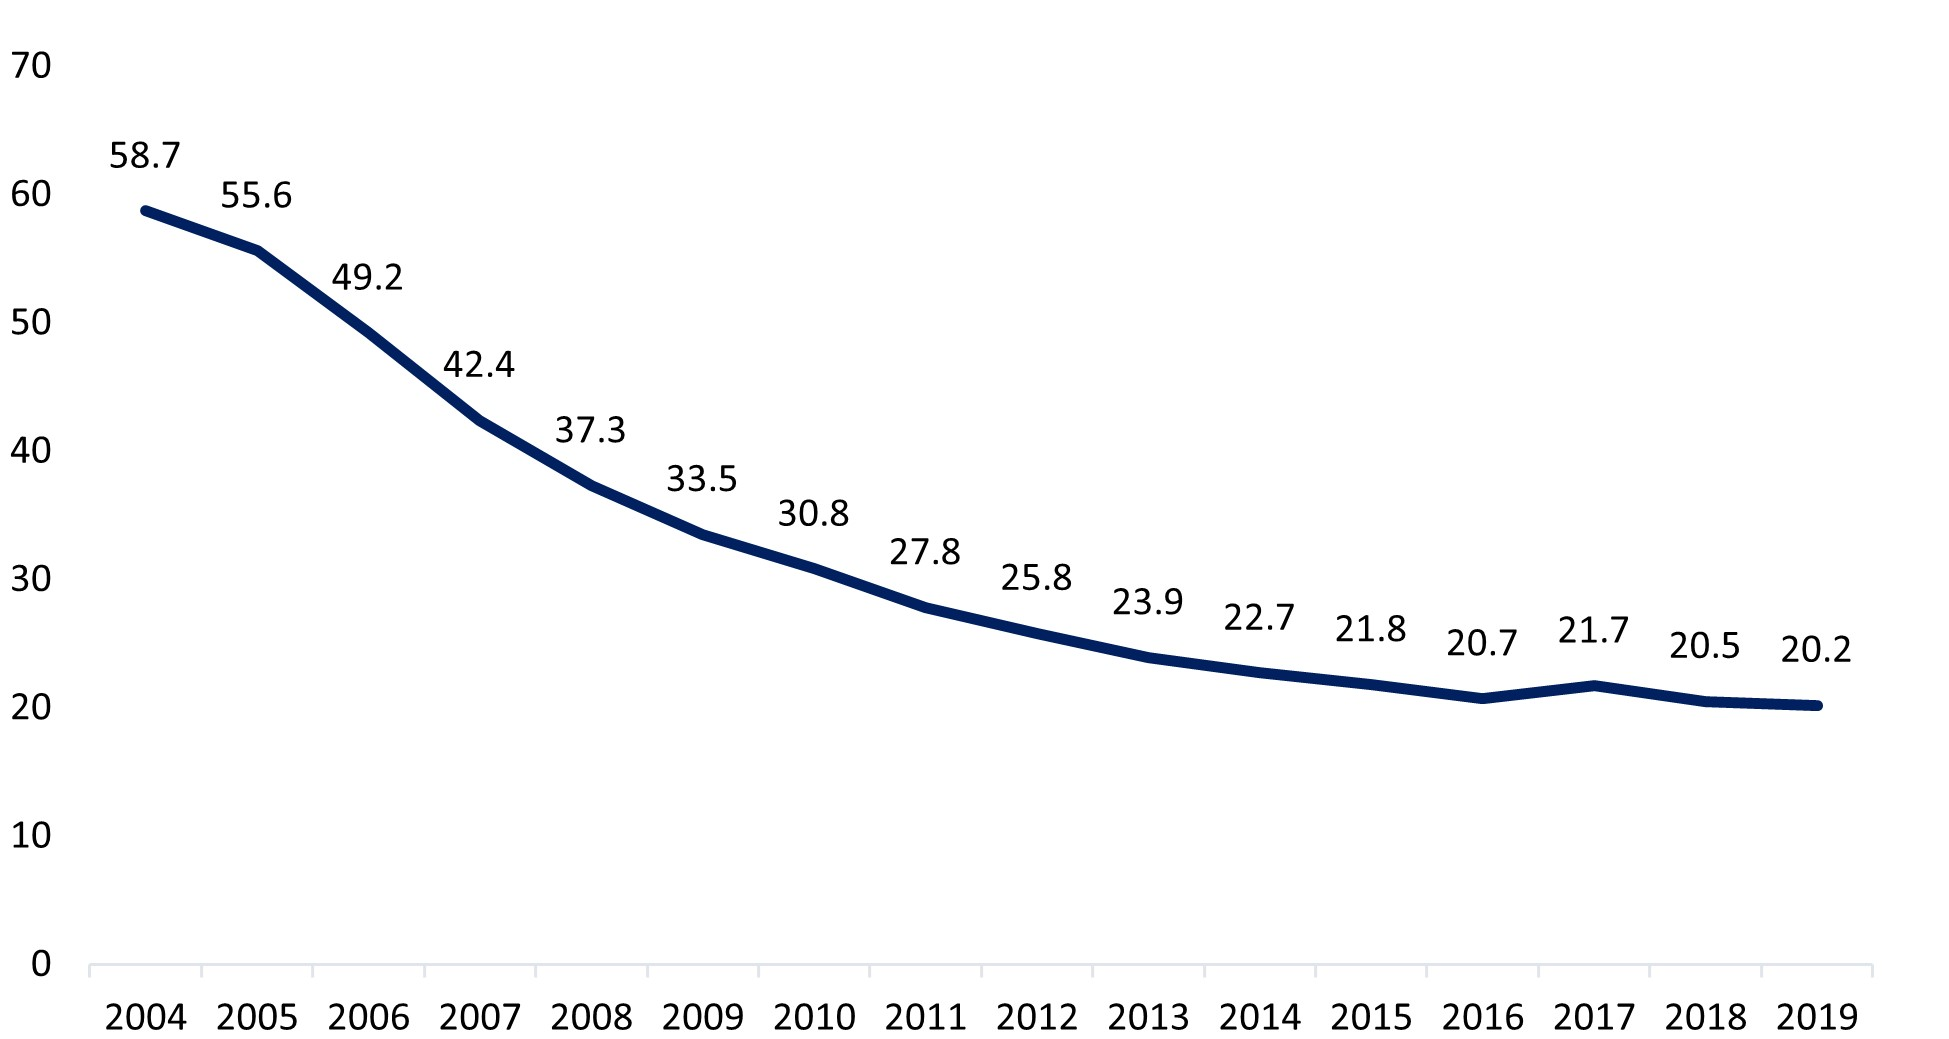
\includegraphics[scale=0.8]{images/chapter1/Imagen1.jpg}
    \label{fig:Figure1}  
    
     \begin{tablenotes}[para,flushleft]
     {\small
         \textit{Note.} Elaboración propia, Banco mundial.
     }
     \end{tablenotes}
\end{figure}

Donde precisa que la tasa de incidencia de la pobreza entre 2004 y 2019 se redujo en 38.5\%. señala también que el principal periodo de reducción fue entre 2004 y 2011. 

Los años 2002 a 2016 la tasa de pobreza bajo de 54,30\% a 20,7\% y la extrema pobreza de 24.2\% a 3.8\%, ya que, en los gobiernos de Alejandro Toledo, Alan García y Ollanta Humana la tasa de pobreza se redujo en 5,2\%, 21,4\%, 7,03\% y la extrema pobreza en 10,4\%, 7,5\%; 2,54\%, respectivamente, llegando para el año 2018 con 20,50\% de pobreza y 2,8\% de extrema pobreza, con predisposición a seguir descendiendo. 

La tasa de pobreza pasó de 54\% en 1990 a 20,50\% para 2018 y la extrema pobreza de 24.2\% a 2.8\% en el mismo periodo de años, reduciéndose significativamente la pobreza y extrema pobreza en 33,5\% y 21.4\% respectivamente; esto como consecuencia del crecimiento económico sostenido, lo cual implicó un aumento del gasto social, aumento de la inversión pública y una mejora en la calidad y focalización de los programas sociales.

En los periodos 2001 a 2010, la pobreza decreció en 23,5 puntos porcentuales, al pasar de 54,8\% a 31,3\% en el 2010.

\begin{figure}[H]
    \caption{Evolución de la tasa de pobreza, 2001-2010 (\% de la población total).}
    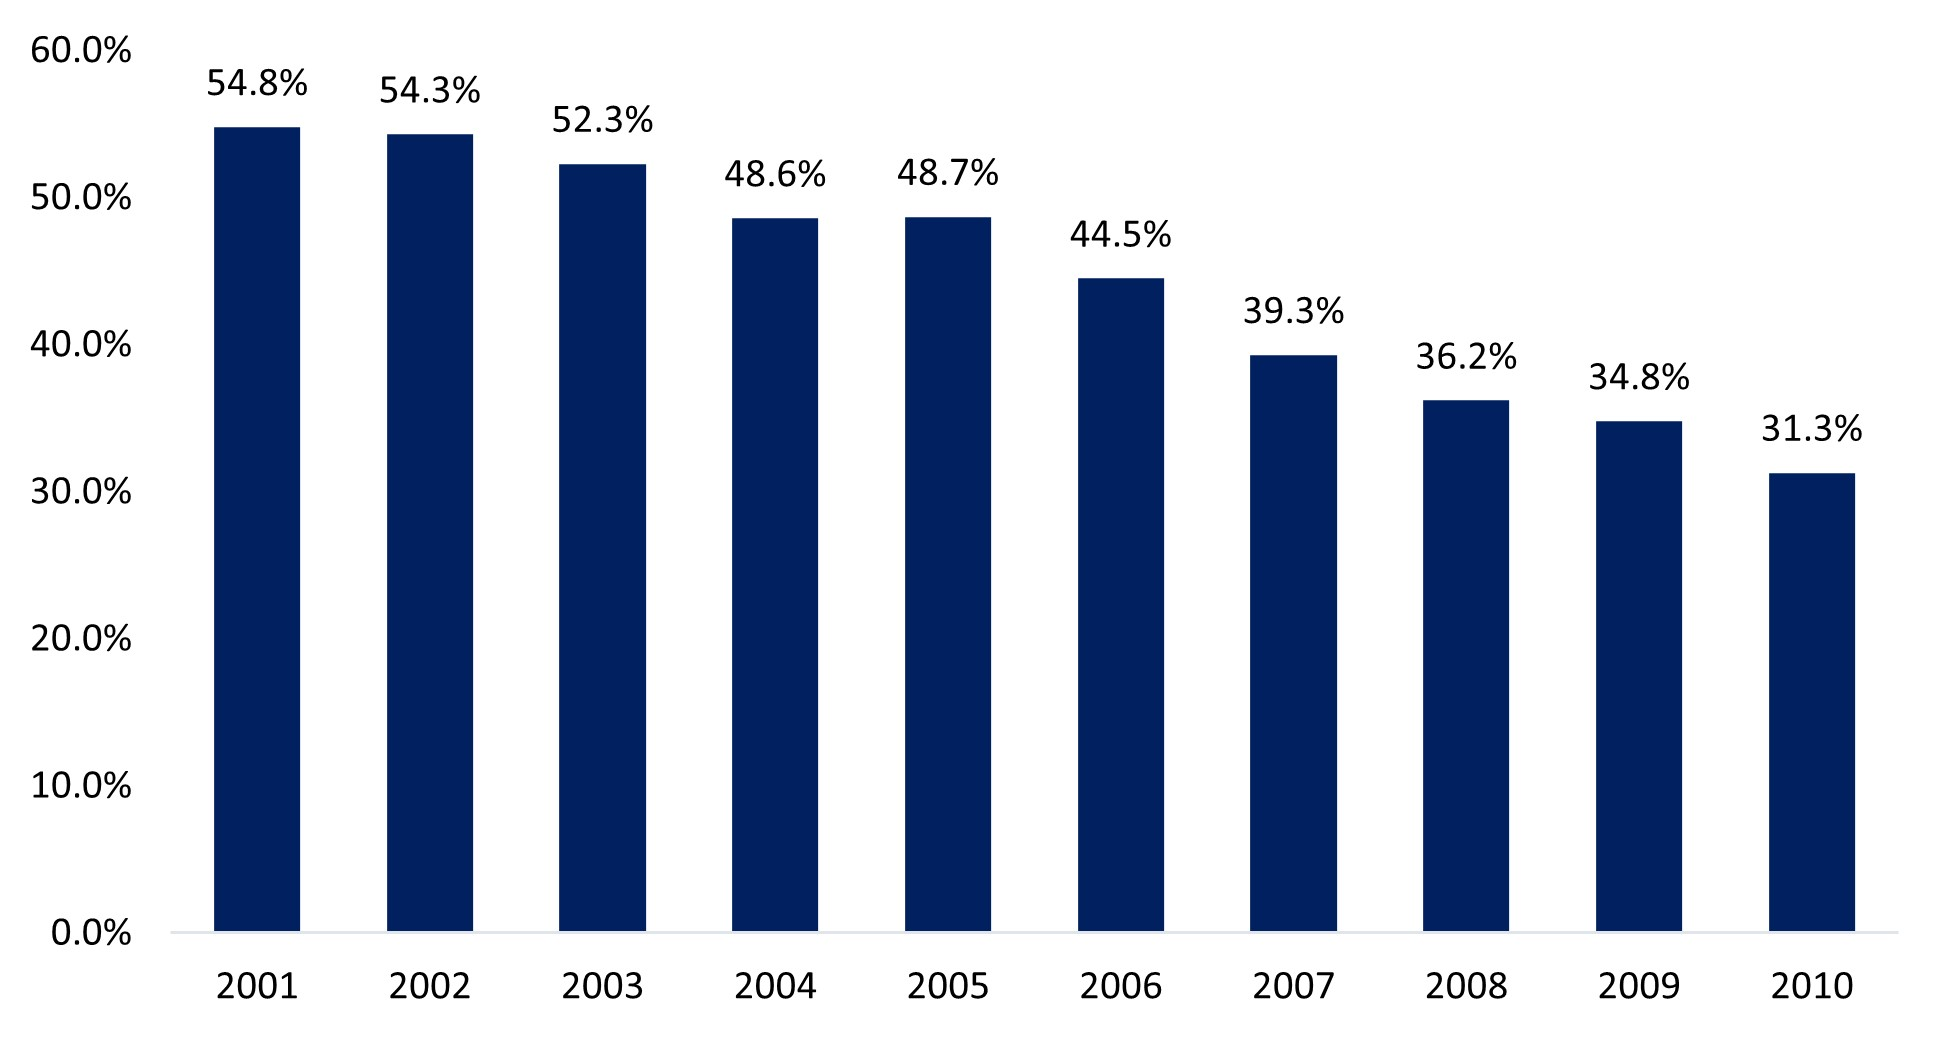
\includegraphics[scale=0.8]{images/chapter1/Imagen2.jpg}
    \label{fig:Figure2}  
    
     \begin{tablenotes}[para,flushleft]
     {\small
         \textit{Note.} Elaboración propia, Banco mundial.
     }
     \end{tablenotes}
\end{figure}

Mientras que en año 2017, 6 millones 906 mil de personas (21,7\%), se encontraban en situación de pobreza, lo que significa que estas personas tenían un nivel de gasto por debajo del costo de la canasta básica de consumo. Comparando este resultado con los niveles del año 2016, se puede observar que la tasa de pobreza ha aumentado en 1,0\%, equivalente a 375.000 pobres, más que en 2016.

\begin{figure}[H]
    \caption{Evolución de la tasa de pobreza, 2001-2010 (\% de la población total).}
    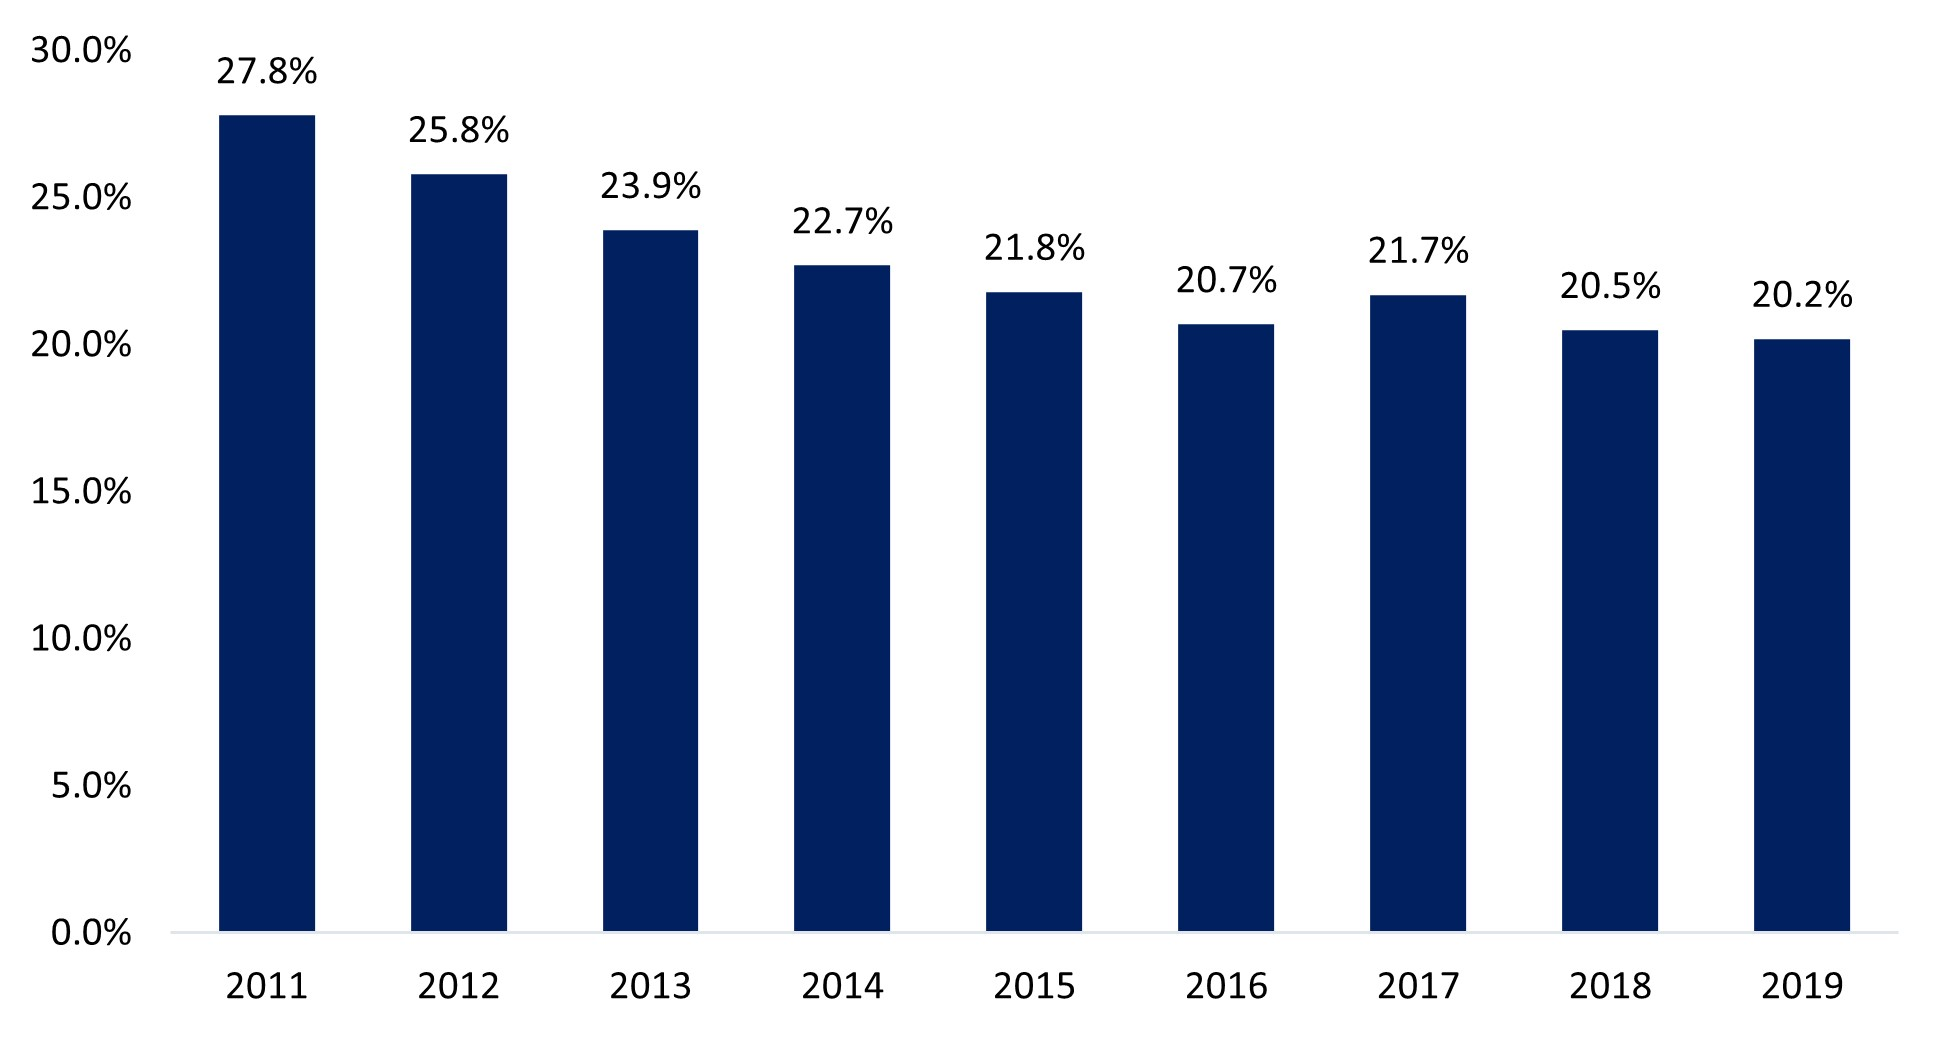
\includegraphics[scale=0.8]{images/chapter1/Imagen3.jpg}
    \label{fig:Figure3}  
    
     \begin{tablenotes}[para,flushleft]
     {\small
         \textit{Note.} Elaboración propia, INEI.
     }
     \end{tablenotes}
\end{figure}

En 2019, el índice de pobreza monetaria afectó al 20,2\% de la población del país, manteniendo casi el mismo nivel que en 2018; Así lo publicó el INEI, de acuerdo con los resultados de la Encuesta Nacional de Hogares (ENAHO) 2019. También señaló que la población en pobreza es considerada la población promedio. el gasto está por debajo del valor de la línea de pobreza (PL), el equivalente monetario de una canasta de productos básicos y alimenticios.

Cuando se habla de pobreza también se hace referencia a la desigualdad social; un grupo social que es excluido ya que no cuenta con el mismo acceso a los recursos que otros grupos con poder si tienen, estas diferencias están marcadas con claridad entre las zonas urbanas y rurales. 

La aplicación errada de políticas públicas ha pronunciado aún más las diferencias, ya que no se ha permitido una integración de la multiculturalidad con la que cuenta el Perú, y muy por el contrario ha ocasionado un marcado distanciamiento entre ellos.

En un contexto de crecimiento económico sostenido, es necesario mejorar la formulación y aplicación de las políticas del país, en objetivos puntuales de desarrollo y asistencia social con el firme objetivo de combatir la pobreza a largo plazo mejorar los estándares de vida de su población en conjunto.


\subsection{Formulación del problema}

\subsubsection{Problema general}

¿Cómo la desigualdad socioeconómica determina el grado de pobreza en el departamento de Ayacucho, periodo 2000-2019?

\subsubsection{Problemas específicos }

\begin{itemize}

\item ¿Cuál es la influencia del empleo en el IDH en el departamento de Ayacucho, periodo 2000-2019?

\item ¿Cuál es la incidencia del índice de Theilen en la determinación de grado de pobreza en el departamento de Ayacucho, periodo 2000-2019?

\item ¿Como el desempleo influye en el índice de Gini en el departamento de Ayacucho, periodo 2000-2019? 

\end{itemize}




	
	% II. OBJETIVOS
	\section{\large OBJETIVOS}

\subsection{Objetivo general}

Establecer cómo de la desigualdad socioeconómica incide en la pobreza en el departamento de Ayacucho, periodo 2000-2019.

\subsection{Objetivos específicos}

\begin{itemize}
\item Analizar cómo el empleo influye en el Índice de Desarrollo Humano en las zonas rurales de Ayacucho.
\item Determinar cuánto el Índice de Theilen influye en el Grado de pobreza.
\item Identificar de qué manera el desempleo determina el índice de Gini en el departamento de Ayacucho.

\end{itemize}


	
	
	


	
		
	% III. JUSTIFICACIÓN
	\section{\large JUSTIFICACIÓN}

\subsection{Justificación teórica}
	
La pobreza es un problema mundial que se ha venido combatiendo a lo largo de los años, cada país en forma individual ha implementado medidas y políticas con el único fin de reducir su nivel de pobreza o extrema pobreza. En caso particular de Perú, a pesar de los índices favorables en la reducción de la pobreza, en determinadas zonas se observa un margen significativo en la desigualdad socioeconómica el cual es paralelo al índice del nivel pobreza.

Es importante analizar el comportamiento de los índices de pobreza contrastado con indicadores de la desigualdad socioeconómica; para así poder establecer efectividad o importancia a lo largo del tiempo. Crear conocimiento dentro de la relación establecida entre estos indicadores, de manera que se contraste con la teoría económica ya conocida o se generen nuevos aportes.


\subsection{Justificación practica}

Este trabajo tiene una justificación practica porque con él podrá ser posible su aplicación a la realidad para poder hacer frente a la desigualdad socioeconómica que predomina en distintas regiones en particular y sobre todo hacer frente a la pobreza que tanto sufrimiento ocasiona a una gran parte de la población peruana. 

Los resultados de la presente investigación podrán aportar a ver mejor el panorama del país y con él se podrán diseñar estrategias de políticas públicas con los que en un mediano plazo podamos obtener resultados más eficaces en la reducción de la pobreza y la desigualdad socioeconómica en el Perú; además del gran aporte que significara para la toma de decisiones a nivel de gobierno.

\subsection{Justificación metodológica}

Para realizar la investigación sobre la influencia de la desigualdad socioeconómica en la pobreza se empleará el método hipotético deductiva, es decir, iremos de los general a lo particular; primero se hará una visión general de la desigualdad socioeconómica y de la pobreza de la región Latinoamérica para posteriormente, estudiar el caso particular de Perú.










		


		
	% IV. MARCO TEORICO
	\section{\large MARCO TEÓRICO}

\subsection{Marco histórico}
	
\subsubsection{Enfoque Subjetivo}

De La Piedra (1984), afirma que la pobreza subjetiva “significa considerar que cualquier individuo o familia puede opinar sobre qué tan bien se están satisfaciendo sus necesidades básicas, en otras palabras, sobre el grado al cual ella misma piensa que sus medios les sirven para alcanzar sus fines”. Por tanto, de acuerdo a este juicio se le considera pobre o no pobre.

\subsubsection{Enfoque Relativo}
Según Townsend (1962), en su enfoque de la privación relativa, “se concibe un umbral del ingreso, de acuerdo con el tamaño y el tipo de familia, por debajo del cual el abandono o la exclusión de la membresía activa de la sociedad se acentúa en forma desproporcionada”. 

Para Murillo Alfaro (1993), “en el enfoque de pobreza relativa, la felicidad de un individuo o de una familia no depende de su nivel absoluto de consumo o gasto, sino de su nivel de logro en las relaciones con otros miembros de la sociedad”. El punto de partida es buscar un punto de referencia que pueda ser una media o un grupo social específico. Así, la pobreza se define como un estado de necesidades básicas insatisfactorias en relación con la sociedad.

\subsubsection{Enfoque absoluto}
Sen (1981), enfatiza que “existe un núcleo innegable de privación absoluta en la idea de pobreza, que conduce a manifestaciones visibles de muerte por hambre, desnutrición y penuria en un diagnóstico de la pobreza, sin tener que indagar primero en un panorama relativo”. Por lo cual, la idea de pobreza relativa integra y no reemplaza el enfoque de pobreza autoritaria.


\subsection{Marco referencial}
	
La desigualad socioeconómica es un tema de poca frecuencia y permanente interés. Según Cotler (2011), en los años de 1960 la forma de pensar sobre la desigualdad socioeconómica estaba influenciado por la sociología funcionalista - estructuralista, así como el Marxismo. 

Así, se puede decir que, en las ciencias sociales peruanas, dos enfoques que pretenden ser "gran teoría" han sido muy influyentes desde la década de 1960: el funcionalismo estructural y el marxismo.

Según Jiménez (2016), la desigualdad es un problema porque afecta a la calidad de vida de las personas y restringe las capacidades y libertades individuales.

Por tanto, la desigualdad se considera como una externalidad negativa donde las personas o familias no están dispuestos a tolerar altos niveles de desigualdad. Figueroa, (2001).

En cuanto a la pobreza, en términos monetarios, alude a la falta de ingresos para poder cubrir el costo de una canasta básica de consumo; por otro lado, la carencia de ingresos suficientes "está asociada a la carencia del capital humano necesario para acceder a ciertos empleos", o a la falta de "capital financiero, tierra y conocimientos gerenciales y tecnológicos para desarrollar una actividad empresarial", CEPAL (2000).

Si hacemos referencia a un enfoque más complejo, analizamos al premio Noble Amartya Sen, quien menciona: "la pobreza debe concebirse como la privación de capacidades básicas y no meramente como la falta de ingresos, que es el criterio habitual con el que se identifica la pobreza" (Sen, 2000).  Además, el autor afirma que "cuanto mayor sea la cobertura de la educación básica y de la asistencia sanitaria, más probable es que incluso las personas potencialmente pobres tengan más oportunidades de vencer la miseria" (Sen, 2000).

Otro enfoque para considerar es el de la ya conocida pobreza humana; este enfoque propuesto por el Programa de las Naciones Unidad para el Desarrollo (PNUD) afirma que "el concepto de pobreza humana considera que la falta de ingreso suficiente es un factor importante de privación humana, pero no el único"; por lo tanto, se debe tener en cuenta que no todo empobrecimiento puede relacionarse únicamente con el ingreso. "Si el ingreso no es la suma total de la vida humana, la falta de ingreso no puede ser la suma total de la privación humana" PNUD (2000).

Para Mendoza y García (2006), la pobreza puede tener cambios más significativos manteniéndose un crecimiento económico, pero también es imprescindible el accionar del Estado en la promoción de equidad de oportunidades de desarrollo de la persona (inversión en capital humano) el cual, en un largo plazo, mediante el incremento de la productividad, favorecerá también al crecimiento económico el cual se hará sostenible de forma automática.

Boragina (2006), en su artículo, afirma que existen tres falacias económicas las cuales en la economía moderna quedan desfasadas absolutamente, él afirma que: la riqueza es dinámica, la producción y distribución son un único fenómeno y que el valor es el que genera trabajo; de esta manera, señala que al aferrarnos a las teorías de la economía antigua estamos perpetuando la pobreza en el mundo.


\subsection{Sistema teórico}

  \subsubsection{Desigualdad Socio económica y la Pobreza}

    \paragraph{Desigualdad socio económica}
La desigualdad socioeconómica es un problema actual, producto del desarrollo desigual entre las diferentes regiones del mundo y la imposición de ciertas ideologías o definiciones, el precio de unas personas en relación con otras. De hecho, la desigualdad socioeconómica está en la raíz de la discriminación, ya que la desigualdad incluye un trato diferente de quienes se encuentran en desventaja económica, social o moral.

    \paragraph{La Pobreza}
Las Naciones Unidas (2021), afirma que “la pobreza va más allá de la falta de ingresos y recursos para garantizar medios de vida sostenibles. Es una cuestión de derechos humanos”. Entre las diferentes manifestaciones de la pobreza se encuentran: el hambre, la desnutrición, la falta de una vivienda digna y el acceso limitado a otros servicios básicos como la salud o la educación.

Para el BID “la pobreza es la privación de bienestar, entendiendo el bienestar un concepto bastante complejo y amplio, y su nivel más básico abarca aspectos como la alimentación, vestido, salud, y vivienda”

Mientras para el Banco Mundial (2018), “la pobreza no solo implica falta de ingresos y consumo: también se manifiesta por bajos niveles de educación, resultados insatisfactorios en salud y nutrición, falta de acceso a servicios básicos.” 

Según INEI, (2007) “la pobreza se define como un grupo de personas que no alcanzan un nivel mínimo de satisfacción para una serie de necesidades básicas relacionadas con la salud, la nutrición, la educación, la vivienda y otros.”


    \paragraph{Medición de la pobreza}

  \subparagraph{Línea de pobreza}

El método de la línea de pobreza del INEI (2007), usa una canasta de bienes y servicios (la canasta estándar de necesidades), cuyo valor per cápita (la línea de pobreza) es equivalente al mínimo necesario para la subsistencia. 

Para la Dirección Provincial de Estadística de la provincia de Buenos Aires (2010), “el método más utilizado en el mundo, a pesar de sus limitaciones, es el Método de la Línea de Pobreza (PL), que utiliza el ingreso o el gasto de consumo como medida de bienestar”, estableciendo así, un valor per cápita de una canasta mínima de consumo necesaria para la supervivencia, es decir, una canasta de factores esenciales de satisfacción, que distingue grados de pobreza.


  \subparagraph{Las necesidades básicas insatisfechas (NBI)}

Este método, INEI (2007), define la pobreza como un grupo de personas que no cumplen con el nivel mínimo de satisfacción para un rango de necesidades básicas relacionadas con la educación, vivienda, salud, nutrición, etc. Es decir, parte de un concepto multidimensional de pobreza considerando distintos aspectos del desarrollo social.

Según el DPE (2010), “la medida de las necesidades básicas insatisfechas (NBI) tiene en cuenta un conjunto de indicadores relacionados con las necesidades estructurales básicas (vivienda, educación, salud, infraestructura pública, etc.) que se necesitan para evaluar el nivel de felicidad de un individuo.”


  \subparagraph{Método integrado}

La Medida Integrada de Pobreza del INEI (2007), no es más que una combinación de los dos métodos y se utiliza esencialmente con la finalidad de identificar a los distintos segmentos de los pobres, entendiendo que se debe poner énfasis en las políticas de reducción de la pobreza. 

DPE (2010), El tercer método, denominado medida de pobreza integrada, combina métodos de línea de pobreza y necesidades básicas insatisfechas. Con este método, la población se fragmenta en cuatro grupos específicos:

\begin{itemize}
\item Los crónicamente pobres son el grupo más vulnerable porque tienen al menos una NBI e ingresos o gastos por debajo de la línea de pobreza. 

\item Los pobres recientes, son aquellas personas cuyas necesidades básicas están satisfechas pero sus ingresos están por debajo de la línea de pobreza. 

\item Pobres por inercia, son los que tienen como mínimo una necesidad básica insatisfecha, pero sus ingresos o gastos están por encima de la línea de pobreza. 

\item Inclusión social, son aquellos que no tienen necesidades básicas insatisfechas y su gasto está por encima de la línea de pobreza.

\end{itemize}

  \subsubsection{Empleo e Índice de Desarrollo Humano (IDH)}
El concepto de pleno empleo de la Organización Internacional del Trabajo (OIT) es el escenario de empleo para todos los que quieren trabajar y lo buscan.

Existen dos tipos de empleo; formal e informal (Serie de Estudios Económicos, 2015). En el empleo formal se encuentran las personas cuyo trabajo y derechos laborales son reconocidos; mientras que el empleo informal es lo contrario, puesto que aunque los trabajadores perciben un pago en remuneracion a su trabajo, estos no reciben el mismo reconocimiento ni los derechos laborales.

Para Ricardo (1959), el principal determinante del empleo era la acumulación del capital, el cual significa el uso excedente para contratar trabajadores asalariados.

El Programa de las Naciones Unidas (2021), ha venido publicando desde hace tres décadas, el Informe sobre Desarrollo Humano, el centra su análisis en el comportamiento del desarrollo a nivel mundial. El IDH es un indicador más confiable que el crecimiento del PBI, pues este último basa su razón solo en el comportamiento del nivel de ingreso, mientras que el IDH considera también otras dimensiones más complejas como nivel de ingreso per cápita, esperanza de vida y el acceso a la educación. 

El PDNU (2021), para una interpretación efectiva del IDH, considera cuatro categorías: 

\begin{itemize}
\item Desarrollo humano muy elevado (mayores a 0.8)
\item Desarrollo humano elevado (entre 0.7 y 0.7999)
\item Desarrollo humano medio (entre 0.55 y 0.6999)
\item Desarrollo humano bajo (menores a 0.55)

\end{itemize}

  \subsubsection{Índice de Theilen y grado de pobreza}

    \paragraph{Índice de Theilen}
Wikipedia, (2021) “El índice de Theilen es una estadística que se utiliza principalmente para medir la desigualdad y otros fenómenos económicos, aunque también se ha utilizado para medir la segregación racial.”
 
Según Castañeda (2013), Esta medida es una aplicación prestada directamente de la física y la teoría de la información, que está bien aceptado entre los investigadores de la desigualdad y durante mucho tiempo ha sido una medida alternativa del coeficiente de Gini.

    \paragraph{Grado de pobreza}

  \subparagraph{Extremo pobre}

Para Damm Arnal (2017), “comprende a las personas cuyos hogares tienen ingresos o consumos per cápita inferiores al valor de una canasta mínima de alimentos.”

\subparagraph{Pobre}

Damm Arnal (2017), define a pobre a “la persona que se encuentra en situación de pobreza si padece al menos una privación social, sus ingresos no son suficientes para adquirir los bienes y servicios que constituyen las canastas básicas alimentarias y no alimentarias.”

  \subparagraph{No pobre}

Se considera no pobres a aquellas personas cuyo ingreso o consumo es suficiente para mantener un nivel de vida elevado o de calidad.

  \subsubsection{Desempleo e Índice de Gini}

    \paragraph{Desempleo}

Según De Gregorio (2007), El desempleo es un indicador importante para medir el desempeño de una economía en términos de actividad, además que siempre es aquella fracción de los que quieren trabajar, pero no consiguen hacerlo.

Para. Pissarides (1990), “existe desempleo a causa de fricciones en el mercado laboral en el proceso de búsqueda de empleo por parte de los trabajadores y de contratación por parte de las firmas.”

\cite{Modigliani1998}, afirman que el desempleo afecta principal y directamente a los trabajadores poco calificados, ya que a medida que disminuye la disponibilidad de empleo, los trabajadores más calificados desplazan a los trabajadores poco calificados; mientras que, si aumenta el empleo ocurre todo lo contario, es decir, los trabajadores calificados obtienen mejores trabajos.


    \paragraph{Clases de desempleo}

  \subparagraph{Desempleo friccional}
Es cuando se tiene libertad para escoger los empleos siempre existen personas que se traslada de un trabajo a otro.

  \subparagraph{Desempleo estructural}
Ocurre cuando con el tiempo se presenta cambios en la estructura de la demanda del consumidor y del avance tecnológico los mismos que alteran la estructura de la demanda global de trabajo.

  \subparagraph{Desempleo cíclico}
Este tipo de desempleo es causado por la fase recesiva del ciclo económico cuando quiebran las empresas con escasa solvencia económico y dejan sin trabajo a muchas personas.

    \paragraph{Índice de Gini}

Para Montero Castellanos (2021), “el coeficiente de Gini es una de las métricas utilizada para orientarnos respecto a la desigualdad económica. Cuanto mayor es el índice de Gini, mayor es la desigualdad de los ingresos en la población.” 

\subsection{Marco conceptual}

  \subsubsection{Desigualdad socioeconómica}
  
  La desigualdad socioeconómica es un problema actual, el cual se origina como resultado a un desarrollo desigual, creando a su vez un concepto falso de superioridad.
  
  \subsubsection{La Pobreza}
  
  Según el método de INEI (2007), se define a la pobreza como un grupo de personas que no cumplen con el nivel mínimo de satisfacción para un rango de necesidades básicas relacionadas con la salud, nutrición, educación, vivienda, etc. Es decir, parte de un concepto multidimensional de pobreza considerando diferentes aspectos del desarrollo social.
  
  \subsubsection{Empleo}
  
  El empleo se define como aquel escenario donde existe trabajo para todas las personas que quieran trabajar o estén buscándolo. Existen dos tipos de empleo: formal (reconocido y con todos los derechos laborales) e informal (no está reconocido y no goza de los derechos laborales).
  
  \subsubsection{Índice de Desarrollo Humano (IDH)}
  
  Es aquel indicador que basa su estudio en dimensiones más complejas, lo cual permite obtener un resultado más confiable; mide el nivel de desarrollo de cada país, y sus principales variables son: el nivel de ingreso per cápita, esperanza de vida y el acceso a la educación. Es aquel indicador que basa su estudio en dimensiones más complejas, lo cual permite obtener un resultado más confiable; mide el nivel de desarrollo de cada país, y sus principales niveles variables son: el nivel de ingreso per cápita, esperanza de vida y el acceso a la educación. 
  
  \subsubsection{Índice de Theilen}
  
  El índice de Theilen es una estadística que se utiliza principalmente para medir la desigualdad y otros fenómenos económicos.
  
Cuando el índice de Theilen es cercano a cero la sociedad es igual mientras el índice se va al infinito la es sociedad es desigual. 


  \subsubsection{Grado de pobreza}
  
\paragraph{Extremo pobre} 
Para Damm Arnal (2017), incluye a las personas cuyos hogares tienen un ingreso per cápita o un nivel de consumo por debajo del valor de una canasta mínima de alimentos.

\paragraph{Pobre}

Según Damm Arnal (2017), una persona se encuentra en situación de pobreza si tiene al menos una carencia social (de las seis enumeradas en el primer párrafo) y su ingreso es insuficiente para adquirir los bienes y servicios que componen la canasta básica alimentaria y no alimentaria.


  \subsubsection{Desempleo}
  
  Modigliani, Fitoussi, Moro, Snower, y Solow (1999), afirman que el desempleo afecta principal y directamente a los trabajadores poco calificados, ya que a medida que disminuye la disponibilidad de empleo, los trabajadores más calificados desplazan a los trabajadores poco calificados; mientras que, si aumenta el empleo ocurre todo lo contario, es decir, los trabajadores calificados obtienen mejores trabajos.
  
  \subsubsection{Índice de Gini}
  
  El coeficiente Gini es un indicador que nos permite medir la desigualdad de los ingresos de la población.
  		

		
	% V. HIPOTESIS
	\section{\large HIPÓTESIS}

\subsection{Hipótesis general}

La desigualdad socioeconómica determina negativamente el grado de pobreza en el departamento de Ayacucho, periodo 2000-2019.

\subsection{Hipótesis especifica}

\begin{itemize}
\item El empleo afecta inversamente al IDH en el departamento de Ayacucho, periodo 2000-2019.

\item El índice de Theilen se relaciona directamente al grado de pobreza en el departamento de Ayacucho, periodo 2000-2019.

\item •	El desempleo influye directamente en el índice de Gini en el departamento de Ayacucho, periodo 2000-2019.

\end{itemize}






		

	
	% VI. VARIABLES E INDICADORES
	\section{\large VARIABLES E INDICADORES}

\subsection{Desigualdad socio-económica y dimensiones}

\subsubsection{Variable causa}

X= Desigualdad socioeconómica \\
Indicadores:
\begin{itemize}
\item Empleo
\item Índice de Theilen
\item Desempleo
\end{itemize}


\subsubsection{Variable efecto}

Y=Pobreza \\
Indicadores:
\begin{itemize}
\item Índice de Desarrollo Humano
\item Grado de pobreza
\item Índice de Gini
\end{itemize}

	
\subsection{Operacionales de variables y dimensiones}

\begin{table}[H]
  \caption{Matriz de consistencia}
  \label{tab:table1}
\begin{tabular}{llllll}
\hline
\multicolumn{1}{|c|}{Variable}                       & \multicolumn{1}{c|}{Definición conceptual}                                                                                                                                                                                                                                                                                                                                                                                                                  & \multicolumn{1}{c|}{Definición operacional} & \multicolumn{1}{c|}{Indicadores} & \multicolumn{1}{c|}{Unidad de medida} & \multicolumn{1}{c|}{Valor final} \\ \hline
\multicolumn{1}{|l|}{X = Desigualdad socioeconómica} & \multicolumn{1}{l|}{La desigualdad socioeconómica es un problema actual, producto del desarrollo desigual entre las diferentes regiones del mundo y la imposición de ciertas ideologías o definiciones, el precio de unas personas en relación con otras. De hecho, la desigualdad socioeconómica está en la raíz de la discriminación, ya que la desigualdad incluye un trato diferente de quienes se encuentran en desventaja económica, social o moral.} & \multicolumn{1}{l|}{}                       & \multicolumn{1}{l|}{}            & \multicolumn{1}{l|}{}                 & \multicolumn{1}{l|}{}            \\ \hline
\multicolumn{1}{|l|}{Y=Pobreza}                      & \multicolumn{1}{l|}{Según el método de INEI (2007), se define a la pobreza como un grupo de personas que no cumplen con el nivel mínimo de satisfacción para un rango de necesidades básicas relacionadas con la salud, nutrición, educación, vivienda, etc. Es decir, parte de un concepto multidimensional de pobreza considerando diferentes aspectos del desarrollo social.}                                                                            & \multicolumn{1}{l|}{}                       & \multicolumn{1}{l|}{}            & \multicolumn{1}{l|}{}                 & \multicolumn{1}{l|}{}            \\ \hline
                                                     &                                                                                                                                                                                                                                                                                                                                                                                                                                                             &                                             &                                  &                                       &                                 
\end{tabular}
   \begin{tablenotes}[para,flushleft]
     {\small
         \textit{Note.} Elaboración propia.
     }
     \end{tablenotes}
\end{table} 



	
	% VII. METODOLOGIA
	\section{\large METODOLOGÍA}

\subsection{Tipo y nivel de investigación}

	\subsubsection{Tipo de investigación}

Por el tipo de investigación, la presente investigación reúne las condiciones metodológicas de una investigación longitudinal según el alcance temporal investigación aplicada, en razón que se utilizaron conocimientos de las ciencias económicas a fin de aplicarlas en desigualad socioeconómica y la pobreza en el departamento Ayacucho, periodo 2000-2019.
	
	\subsubsection{Nivel de investigación}
De acuerdo a la naturaleza del estudio de la investigación reúne por su nivel las características de un estudio descriptivo explicativo y correlacional.

\subsection{Población y muestra}
 
	\subsubsection{Población}
	Según Córdova (2006), la población o universo es la totalidad de personas u objetos que tienen una o más características medibles o contables de naturaleza cualitativa o cuantitativa.\\
Para Hilario (2020), la población es un conjunto de elementos que posee características similares.


	\subsubsection{Muestra}
	
\subsection{Fuentes de información}

Los datos usados son de nivel secundario, es decir, son datos ya procesados. Se ha recurrido a la información brindada por las páginas del INEI y BCRP, pues son las instituciones que han venido desarrollando diferentes encuestas y estudios a lo largo de los años y han consignado datos fidedignos los cuales pueden emplearse en todo tipo de investigación que lo requiera.

\subsection{Diseño de investigación}

Para el diseño de nuestra investigación emplearemos un tipo de investigación no experimental, el cual a su vez es longitudinal porque nuestra variable se estudia para determinar o evolución en el tiempo.

\subsection{Técnicas e instrumentos}

	\subsubsection{Técnicas}
	Las principales técnicas que se utilizaran en esta investigación para el análisis de series de tiempo son:
	\begin{itemize}
	\item Las metodologías econométricas y 
    \item estadística inferencial

    \end{itemize}		
	
	\subsubsection{Instrumentos}
	Los principales instrumentos que se aplicarán en las técnicas son:
	
    \begin{itemize}
    \item Stata
    \item Excel
    \item Eviews

    
    \end{itemize}	



		

	
	\newpage
	% VIII. REFERENCIAS BIBLIOGRÁFICAS
	% Referencias
\renewcommand\refname{\large\textbf{REFERENCIAS BIBLIOGRÁFICAS}}
\bibliography{References/references.bib}


% CONCLUSIONES
\cleardoublepage\phantomsection\addcontentsline{toc}{section}{\bf \large CONCLUSIONES}
\section*{\centerline {CONCLUSIONES}}
\markboth{CONCLUSIONES}{}
%--
\begin{enumerate}

\item Nam dui ligula, fringilla a, euismod sodales, sollicitudin vel, wisi.  Morbiauctor lorem non justo. Nam lacus libero, pretium at, lobortis vitae, ultricies et,tellus. Donec aliquet, tortor sed accumsan bibendum, erat ligula aliquet magna,vitae ornare odio metus a mi.

\item Nam dui ligula, fringilla a, euismod sodales, sollicitudin vel, wisi.  Morbiauctor lorem non justo. Nam lacus libero, pretium at, lobortis vitae, ultricies et,tellus. Donec aliquet, tortor sed accumsan bibendum, erat ligula aliquet magna,vitae ornare odio metus a mi.

\item Nam dui ligula, fringilla a, euismod sodales, sollicitudin vel, wisi.  Morbiauctor lorem non justo. Nam lacus libero, pretium at, lobortis vitae, ultricies et,tellus. Donec aliquet, tortor sed accumsan bibendum, erat ligula aliquet magna,vitae ornare odio metus a mi.


\end{enumerate}

	
% RECOMENDACIONES	
\cleardoublepage\phantomsection\addcontentsline{toc}{section}{\bf \large RECOMENDACIONES}
\section*{\centerline {RECOMENDACIONES}}
\markboth{RECOMENDACIONES}{}
%
\begin{enumerate}
\item Nam dui ligula, fringilla a, euismod sodales, sollicitudin vel, wisi.  Morbiauctor lorem non justo. Nam lacus libero, pretium at, lobortis vitae, ultricies et,tellus. Donec aliquet, tortor sed accumsan bibendum, erat ligula aliquet magna,vitae ornare odio metus a mi.

\item Nam dui ligula, fringilla a, euismod sodales, sollicitudin vel, wisi.  Morbiauctor lorem non justo. Nam lacus libero, pretium at, lobortis vitae, ultricies et,tellus. Donec aliquet, tortor sed accumsan bibendum, erat ligula aliquet magna,vitae ornare odio metus a mi.

\item Nam dui ligula, fringilla a, euismod sodales, sollicitudin vel, wisi.  Morbiauctor lorem non justo. Nam lacus libero, pretium at, lobortis vitae, ultricies et,tellus. Donec aliquet, tortor sed accumsan bibendum, erat ligula aliquet magna,vitae ornare odio metus a mi.


\end{enumerate}
	
% ANEXOS	

	
\end{document}